\section{Afstandsmåler}

For at sikre dronen under flyvning er det besluttet der skal tilføjes minimum to afstandsmålere. En af afstandsmålerne skal bruges til at måle flyvehøjde og en til antikollision.

Det er vigtigt at dronen på ethvert tidspunkt under flyvning kender egen flyvehøjde. Dette vil sikre dronen hverken flyver for højt eller for lavt. Desuden er det vigtigt at dronen kan detektere eventuelle forhindringer og manøvre udenom dem.

Afstandsmålere vælges ud fra følgende kriterier:  
\begin{itemize}
	\item Pris.
	\item Rækkevide. 
	\item Størrelse/vægt. 
\end{itemize}

\vspace{0.5cm}

Følgende 3 slags sensorer blev overvejet som afstandsmålere. 
\newline Ultralyds afstandsmåler - HC-SR04\footnote{http://www.hobbyking.com/hobbyking/store/RC\textunderscore PRODUCT\textunderscore SEARCH.asp?strSearch=HC-SR04}  
\newline IR afstandsmåler - Sharp GP2Y0A710K0F\footnote{http://www.adafruit.com/products/1568}  \newline Laser afstandsmåler - LIDAR-Lite\footnote{https://store.3drobotics.com/products/lidar-lite}  \newline Se tabel \ref{tab:Afstands_sensorer} for kort sensor sammenligning.

\begin{table}[H]
	\centering
		\begin{tabular}{|p{2.8cm}|p{3.4 cm}|p{3.4 cm}|p{3.4 cm}|} 
		\hline
			\textbf{Specifakation} 	& \textbf{Ultralyds sensor} 	& \textbf{Ir sensor} 		& \textbf{Laser sensor} \\ \hline
			 Forsyning 				& DC 5V 						& DC 5V 					& DC 5V \\ \hline			 
			 Output 				& Puls, \newline skiftede bredde 		& Spænding \newline 1.4 - 3.4V 		& PWM, \newline skiftede duty cycle\\ \hline
			 Rækkevide 					& 0.02 - 4.5m 					& 1.0 - 5.0m 				& 1.0 - 40.0m \\ \hline
			 Vægt 					& 8,5 gram 						& 11 gram 					& 12 gram \\ \hline
		 	 Pris 					& 20 kr 						& 150 kr 					& 450 kr \\ \hline			 
		\end{tabular}
	\caption{Afstands sensorer}
	\label{tab:Afstands_sensorer}
\end{table}

\vspace{0.5cm}

Ud fra kriterierne blev det besluttet at gøre brug af ultralyds sensoren HC-SR04 til både højdemåling og antikollision. HC-SR04 blev valgt da: Ingeniørhøjskolen havde nogle HC-SR04 tilgængelig for udlån, og fordi HC-SR04 er en meget billig afstandsmåler. Hvilket betyder der der nemt kan købes nye/flere sensorer. Desuden har HC-SR04 sensoren en tilpas rækkevide og et simpelt 4 wires interface. 

\begin{figure}[H]
\centering
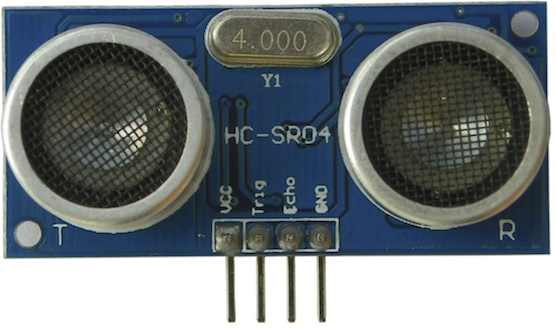
\includegraphics[width=0.3\textwidth]{Billeder/Afstandsmaler/ultra_sensor.png}
\caption{HC-SR04}
\label{fig:HC-SR04}
\end{figure}

\newpage

HC-SR04 aktiveres ved at modtage en trigger puls på minimum 10 \text{µ-sekunder.}
Herefter udsender sensoren 8 bursts af 40khz lydsignal fra sin sender. Efter udsending af de 8 bursts sættes echo-benet logisk højt. Når et burst rammer et objekt reflekteres lydsignalet tilbage til HC-SR04 og rammer modtager delen - hvilket sætter echo-benet lavt. Ved at måle pulsbredden på echo-benet kan afstanden til et objekt udregnes. 

Afstand til objekt kan beregnes på følgende vis: $pulsbredde * lydenshastighed * 0.5$

\vspace{0.2cm}

\begin{figure}[H]
\centering
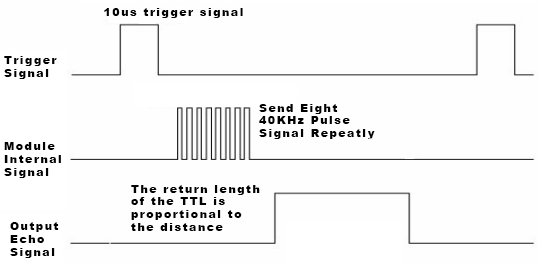
\includegraphics[width=1\textwidth]{Billeder/Afstandsmaler/ultra_schematic.png}
\caption{HC-SR04}
\label{fig:HC-SR04}
\end{figure}

\vspace{2cm}








